The prediction of $Y(\theta)$ conditional on the six evaluation points is shown in figure \ref{2cPred}. Furthermore, the probability that $Y(\theta)<0.30$ conditional on these points is shown in figure \ref{2cTheta}. 

In figure \ref{2cTheta} it appears that the probabilty of $Y(\theta)<0.30$  is maximal at $\theta = 0.36$ with $\text{Pr}\{Y(\theta=0.36)<0.30\}=0.18$. Although there also appears to be a relatively high value for $\text{Pr}\{Y(\theta)<0.30\}=0.15$ for $\theta=0.25$, figure \ref{2cPred} shows that there is much higher variance at $\theta=0.25$ than at $\theta = 0.36$. We would therefore suggest that the scientist use $\theta = 0.36$ to maximize their chances of achieving $Y(\theta)<0.30$.

\begin{figure}
    \centering
    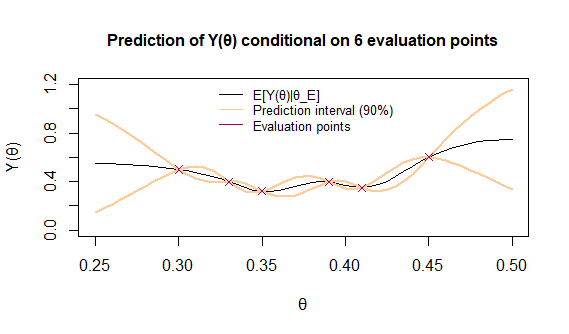
\includegraphics[width=100mm]{2cPred.png}
    \caption{Prediction of $Y(\theta)$ conditional on the six evaluation points  ($\theta$, $y(\theta)$): $(0.30,0.5)$, $(0.33, 0.40)$, $(0.35,0.32)$, $(0.39,0.40)$, $(0.41,0.35)$, and $(0.45,0.60)$. The graph includes a $90\%$ prediction interval. }
    \label{2cPred}
\end{figure}
\begin{figure}
    \centering
    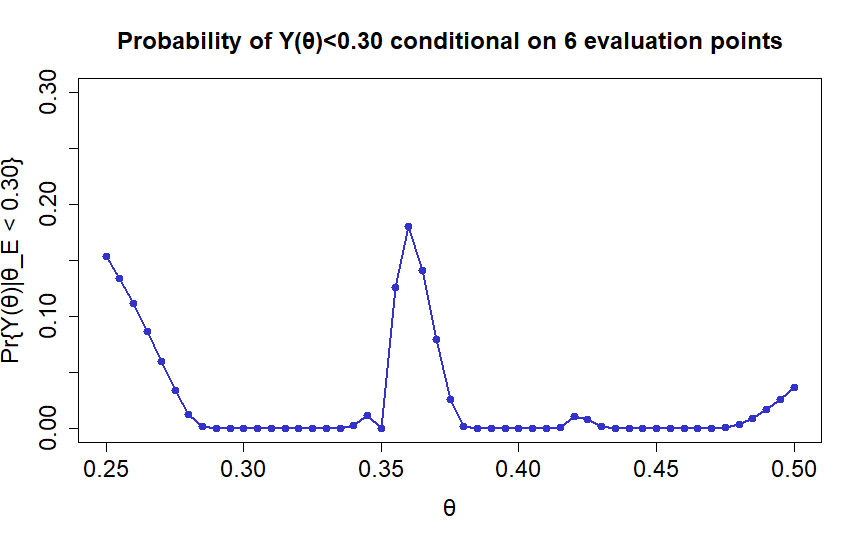
\includegraphics[width=100mm]{2ctheta.png}
    \caption{The probability of $Y(\theta)<0.30$ conditional on the six evaluation points ($\theta$, $y(\theta)$): $(0.30,0.5)$, $(0.33, 0.40)$, $(0.35,0.32)$, $(0.39,0.40)$, $(0.41,0.35)$, and $(0.45,0.60)$.}
    \label{2cTheta}
\end{figure}
